% LaTeX Template für Abgaben an der Universität Stuttgart
% Autor: Sandro Speth
% Bei Fragen: Sandro.Speth@iste.uni-stuttgart.de
%-----------------------------------------------------------
% Hauptmodul des Templates: Hier können andere Dateien eingebunden werden
% oder Inhalte direkt rein geschrieben werden.
% Kompiliere dieses Modul um eine PDF zu erzeugen.

% Dokumentenart. Ersetze 12pt, falls die Schriftgröße anzupassen ist.
\documentclass[12pt]{scrartcl}
% Einbinden der Pakete, des Headers und der Formatierung.
% Mit den \include und \input Befehlen können Dateien eingebunden werden:
% \include: Fügt einen Seitenumbruch nach dem Text ein
% \input: Fügt KEINEN Seitenumbruch nach dem Text ein
% LaTeX Template für Abgaben an der Universität Stuttgart
% Autor: Sandro Speth
% Bei Fragen: Sandro.Speth@iste.uni-stuttgart.de
%-----------------------------------------------------------
% Modul fuer verwendete Pakete.
% Neue Pakete einfach einfuegen mit dem \usepackage Befehl:
% \usepackage[options]{packagename}
\usepackage[utf8]{inputenc}
\usepackage[T1]{fontenc}
\usepackage[ngerman]{babel}
\usepackage{lmodern}
\usepackage{graphicx}
\usepackage[pdftex,hyperref,dvipsnames]{xcolor}
\usepackage{listings}
\usepackage[a4paper,lmargin={2cm},rmargin={2cm},tmargin={3.5cm},bmargin = {2.5cm},headheight = {4cm}]{geometry}
\usepackage{amsmath,amssymb,amstext,amsthm}
\usepackage[lined,algonl,boxed]{algorithm2e}
% alternative zu algorithm2e:
%\usepackage[]{algorithm} %counter mit chapter
%\usepackage{algpseudocode}
\usepackage{tikz}
\usepackage{hyperref}
\usepackage{url}
\usepackage[inline]{enumitem} % Ermöglicht ändern der enum Item Zahlen
\usepackage[headsepline]{scrlayer-scrpage} 
\usepackage{hhline}
\pagestyle{scrheadings} 
\usetikzlibrary{automata,positioning}

% LaTeX Template für Abgaben an der Universität Stuttgart
% Autor: Sandro Speth
% Bei Fragen: Sandro.Speth@iste.uni-stuttgart.de
%-----------------------------------------------------------
% Modul beinhaltet Befehl fuer Aufgabennummerierung,
% sowie die Header Informationen.

% Überschreibt enumerate Befehl, sodass 1. Ebene Items mit
\renewcommand{\theenumi}{(\alph{enumi})}
% (a), (b), etc. nummeriert werden.
\renewcommand{\labelenumi}{\text{\theenumi}}

% Counter für das Blatt und die Aufgabennummer.
% Ersetze die Nummer des Übungsblattes und die Nummer der Aufgabe
% den Anforderungen entsprechend.
% Gesetz werden die counter in der hauptdatei, damit siese hier nicht jedes mal verändert werden muss
% Beachte:
% \setcounter{countername}{number}: Legt den Wert des Counters fest
% \stepcounter{countername}: Erhöht den Wert des Counters um 1.
\newcounter{sheetnr}
\newcounter{exnum}

% Befehl für die Aufgabentitel
\newcommand{\exercise}[1]{\section*{Aufgabe \theexnum\stepcounter{exnum}: #1}} % Befehl für Aufgabentitel

% Formatierung der Kopfzeile
% \ohead: Setzt rechten Teil der Kopfzeile mit
% Namen und Matrikelnummern aller Bearbeiter
\ohead{Oliver Löhr (3311903) Bachelor Informatik \\
        Lara Aziz (3720604) Bachelor Informatik \\
        Joel Thomas (3814387) Master Computer Science} \\

% \chead{} kann mittleren Kopfzeilen Teil sezten
% \ihead: Setzt linken Teil der Kopfzeile mit
% Modulnamen, Semester und Übungsblattnummer
\ihead{Foundations of Artificial Intelligence\\
Wintersemester 2025/26\\
Assignment 1}


% Counter für das Blatt und die Aufgabennummer.
% Ersetze die Nummer des Übungsblattes und die Nummer der Aufgabe
% den Anforderungen entsprechend.
% Definiert werden die Counter in FormatAndHeader.tex
% Beachte:
% \setcounter{countername}{number}: Legt den Wert des Counters fest
% \stepcounter{countername}: Erhöht den Wert des Counters um 1.
\setcounter{sheetnr}{1} % Nummer des Übungsblattes
\setcounter{exnum}{1} % Nummer der Aufgabe

% Beginn des eigentlichen Dokuments
\begin{document}
% Nutze den \exercise{Aufgabenname} Befehl, um eine neue Aufgabe zu beginnen.
% Möchtest du eine Aufgabe in der Nummerierung überspringen, schreibe vor der Aufgabe: \stepcounter{exnum}
% Möchtest du die Nummer einer Aufgabe auf eine beliebige Zahl x setzen, schreibe vor der Aufgabe: \setcounter{exnum}{x}

\section*{1) True or False?}
     \subsection*{a) False}
    An agent does not need complete information about the environment in order to behave rationally.   Rationality is defined relative to the information available to the agent. Even with partial  perception, an agent can
    still choose the action that maximizes expected performance based on what it has observed and what it knows.
    Example: A vacuum cleaner robot may not know the exact layout of a house but can still act rationally by selecting actions that best achieve its cleaning goal given its limited sensors.

    \subsection*{b) True}
     A simple reflex agent bases its decisions only on the current percept and ignores history. However, some environments require memory or state inference for rational behavior.   
     Example: Consider a maze where two distinct locations produce identical sensor readings. The correct action depends on the previous path taken. Since a reflex agent cannot distinguish between these states based solely
     on the current percept, it cannot act rationally in such an environment.

    \subsection*{c) True}
    Such environments can be constructed trivially.
    Example: Imagine an environment with only one state and a performance measure that assigns the
    same score to every action. Since no action can be better or worse than another, any possible
    agent behaves rationally in this setting.

    \subsection*{d) False}
    Agent functions map percept sequences to actions. The set of possible agent functions is uncountably infinite, while the set of computer programs is only countably infinite. Therefore, there are more agent functions
    than programs, which means some agent functions cannot be implemented by any program. Additionally, some functions are not computable at all because they would require solving undecidable problems (e.g., variants of
    the Halting Problem).
    
    \subsection*{e) False}
    Rationality does not imply guaranteed success in every single round, especially in games involving probability and hidden information. A rational agent selects actions that maximize expected utility, but outcomes can
    still be unfavorable due to chance.
    Example: A rational poker agent may go all-in with a statistically strong hand and still lose due to random card draws. Rational play maximizes long-term winnings, but it does not eliminate the possibility of short
    term losses.

\section*{2) Describing Environment Properties of Agents}
    \subsection*{a) Task Environment Selection}
        I have chosen autonomous underwater exploration as my task environment. 
        This is done via autonomous underwater vehicles (AUVs), 
        which are unmanned, untethered vehicles used to conduct underwater research.
        They are equiped with several different sensors and can be programmed to fulfill various tasks.

    \subsection*{b) Observable}
        AUVs are mainly used to explore the sea floor or specific sites and has to rely on its sensors, like cameras and sonar.
        Because only the environment directly observed by the AUV is known, it is only partially observable.
    
        \subsection*{c) Agents}
        In a mission is usually only a single AUV involved, at least in the immediate vicinity. It is therefore a single agent setting.
        
    \subsection*{d) Deterministic Nature}
        The environment is stochastic as every action taken by the agent is subject to random chance. 
        As an example could a changing current change the position of the AUV or a fish swimming past it be picked up by its sensors.
    
    \subsection*{e) Episodic vs. Sequential}
        It is a sequential environment because every action taken by the AUV has an impact on its future actions, 
        for example has every change in position, rotation or velocity an impact on its further navigation.

    \subsection*{f) Dynamic Characteristic}
        The environment is dynamic, as the AUV has to navigate the sea, which changes regardless of the action or inaction of the vehicle.

    \subsection*{g) Discreteness}
        As the environment of underwater exploration is the continuously changing sea, it is a continuous environment.

\section*{3) Agent Functions vs Agent Programs}
    \subsection*{a)}
        Yes, there can be more than one agent program that implements a given agent function. 
        This is possible because we can use different data structures or algorithms to implement the same agent function.
        In the example of the vacuum cleaner where it cleans if there is dirt on the sqare, else moves to the next square, there are numerous ways to implement this solution.
        One method can be by using an if-else statement program - if the square is dirty clean, else move to the next square.
        And another method can be by using a switch case or a lookup table program - read the state of a square and then perfrom the action related to the state in the table.

    \subsection*{b)}
        Yes, there are agent functions that cannot implemented by any agent programs.
        Some of them are agent functions where the decision is made based on an infinite percept history or with infinite memory consumption.
        Another case is when the agent function is computationally expensive that exceeds the limit of the machines.
        And another case is when the solution for a problem cannot be executed mathematically.

    \subsection*{c)}
        The architecture stores the agent programs in the form of 0's and 1's.
        Therefore, the number of distinct agent programs that an n bit storage architecture can have is atmost $2^{n}$.
        The reason for using atmost is that the n bit storage can also store the percept history which maybe required for some of the agent programs.
        Still, the number of configurations of percept and program remains the same, i.e. $2^{n}$.

\section*{4) Two Friends}
    \subsection*{a)Detailed Formulation}
        \subsubsection*{i) State Space}
            The state space should show the current positions of the two friends.
            \[ S = \{(a,b) \mid a,b \in \text{Cities}\}\]
        \subsubsection*{ii) Successor Function}
            The successor function should return all the possible states that can be reached from the current state.
            \[\text{Successor}((a, b)) = \{(a', b') \mid a' \in \text{Neighbors}(a),\; b' \in \text{Neighbors}(b)\}\]
        \subsubsection*{iii) Goal}
            The goal is that both the friends shoud be in the same city, i.e. a = b.
            \[\text{Goal}((a, b)) \colon a = b\]
        \subsubsection*{iv) Step-cost Function}
            The step cost function will be the maximum of the distance that each friend should travel in a single iteration.
            \[\text{Cost}((a, b),(a', b')) = \text{max}(d(a, a'), d(b, b'))\]

    \subsection*{b) Heuristic Functions}
        A heuristic function h(f) is admissable iff,
        \[h(f) \le h'(f)\]
        where h'(f) is the true optimal distance.
        \subsubsection*{i) D(i, j)}
            In this case D(i, j) is admissable as the displacement is always less than or eqaul to the optimal distance between two cities.
            \[D(i, j) \le h'(f)\]
        \subsubsection*{ii) 2.D(i, j)}
            In this case the heuristic function is not admissable as it can be greater than the optimal distance.
            \[2.D(i, j) > h'(f)\]
        \subsubsection*{iii) D(i, j)/2}
            In this case the heuristic function is admissable as dividing the lower value will always be lesser than the optimal value.
            \[D(i, j)/2 \le h'(f)\]

    \subsection*{c) An example where no solution exists}
        An example for a completely connected map where no solutions exists is the case where there are only 2 states (say A and B).
        Since they start in adjacent cities and there is only one other state city that they can go to, they will never meet.
        Therefore, no solution exists for this problem.

    \subsection*{d) Modification of the map for the previous promblem}
        The only way for the above map to have a solution, while being completely connected is by adding one more city to the map.
        In this way, since they always start on adjacent cities, they can always meet at the third city.

    \subsection*{e) Map in which all solutions requireing one friend to visit the same city twice}
        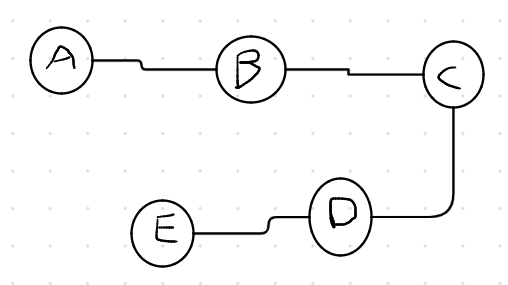
\includegraphics[width=\textwidth]{FAI 4.png}
        In the above map if the friends were to start from adjacent cities (say B and C), both of them would have to visit one city twice in all solutions.
        But there are no maps where only one friend visits the same city twice in all solutions.

\section*{5) Binary tree traversals}
    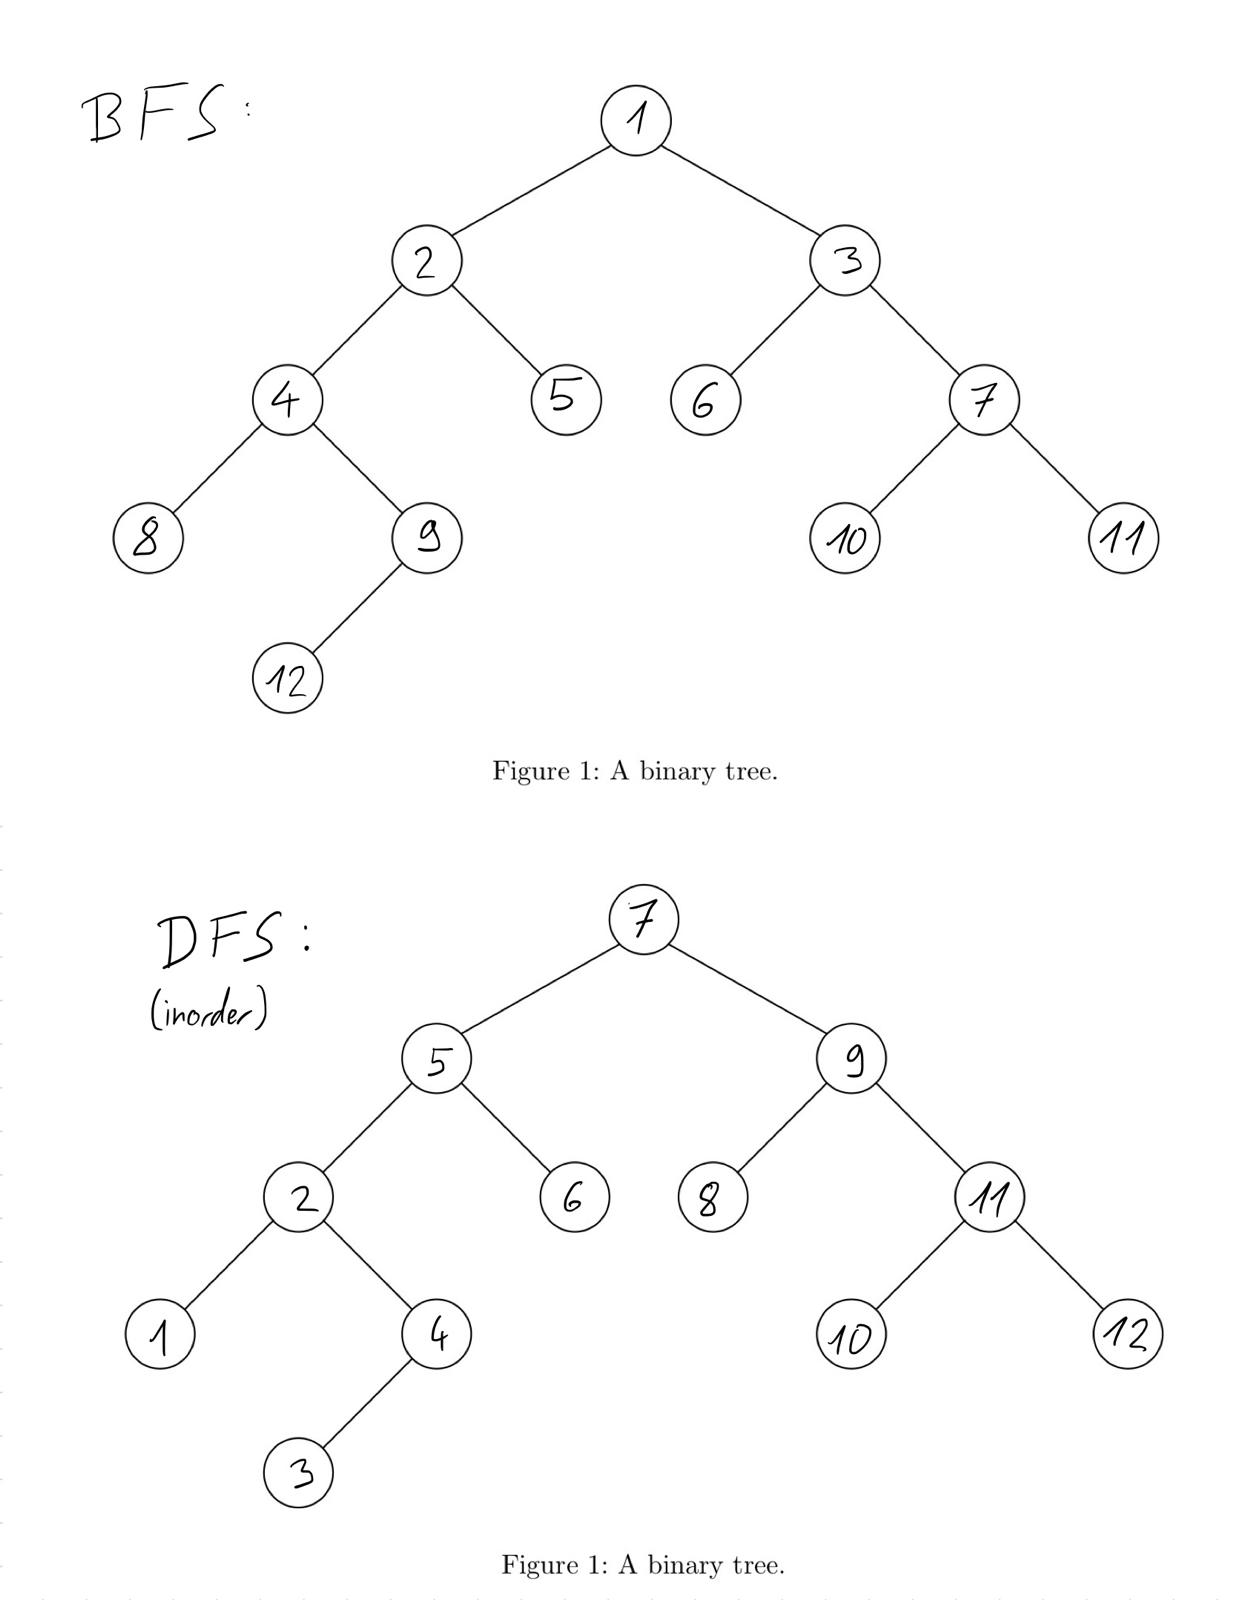
\includegraphics[width=\textwidth]{FAI 1.5.jpeg}

\section*{6) Graph traversals}
    \subsection*{a) BFS}
    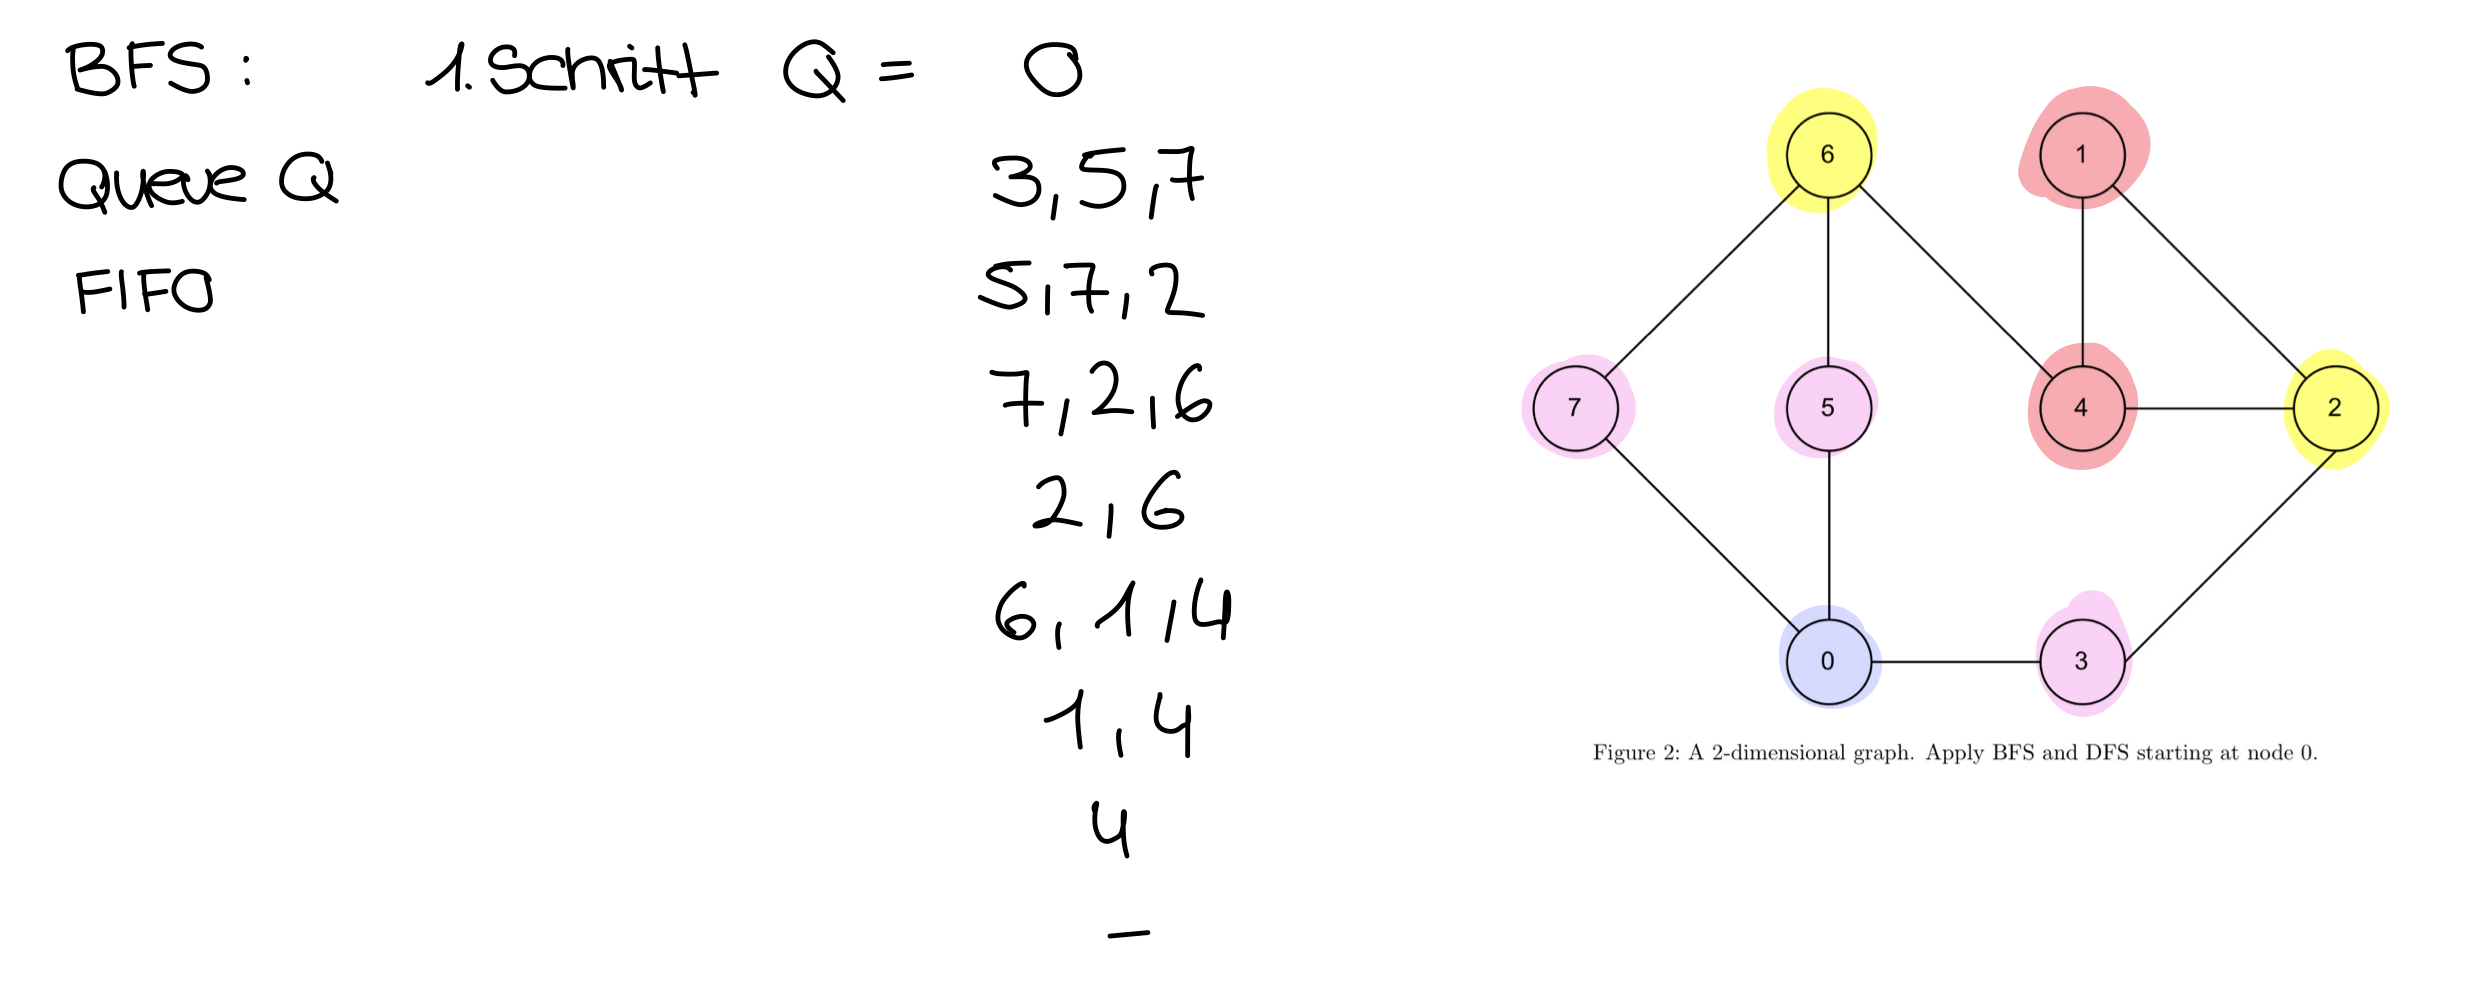
\includegraphics[width=\textwidth]{FAI6a.png}

    \subsection*{b) DFS - lowest value first}
    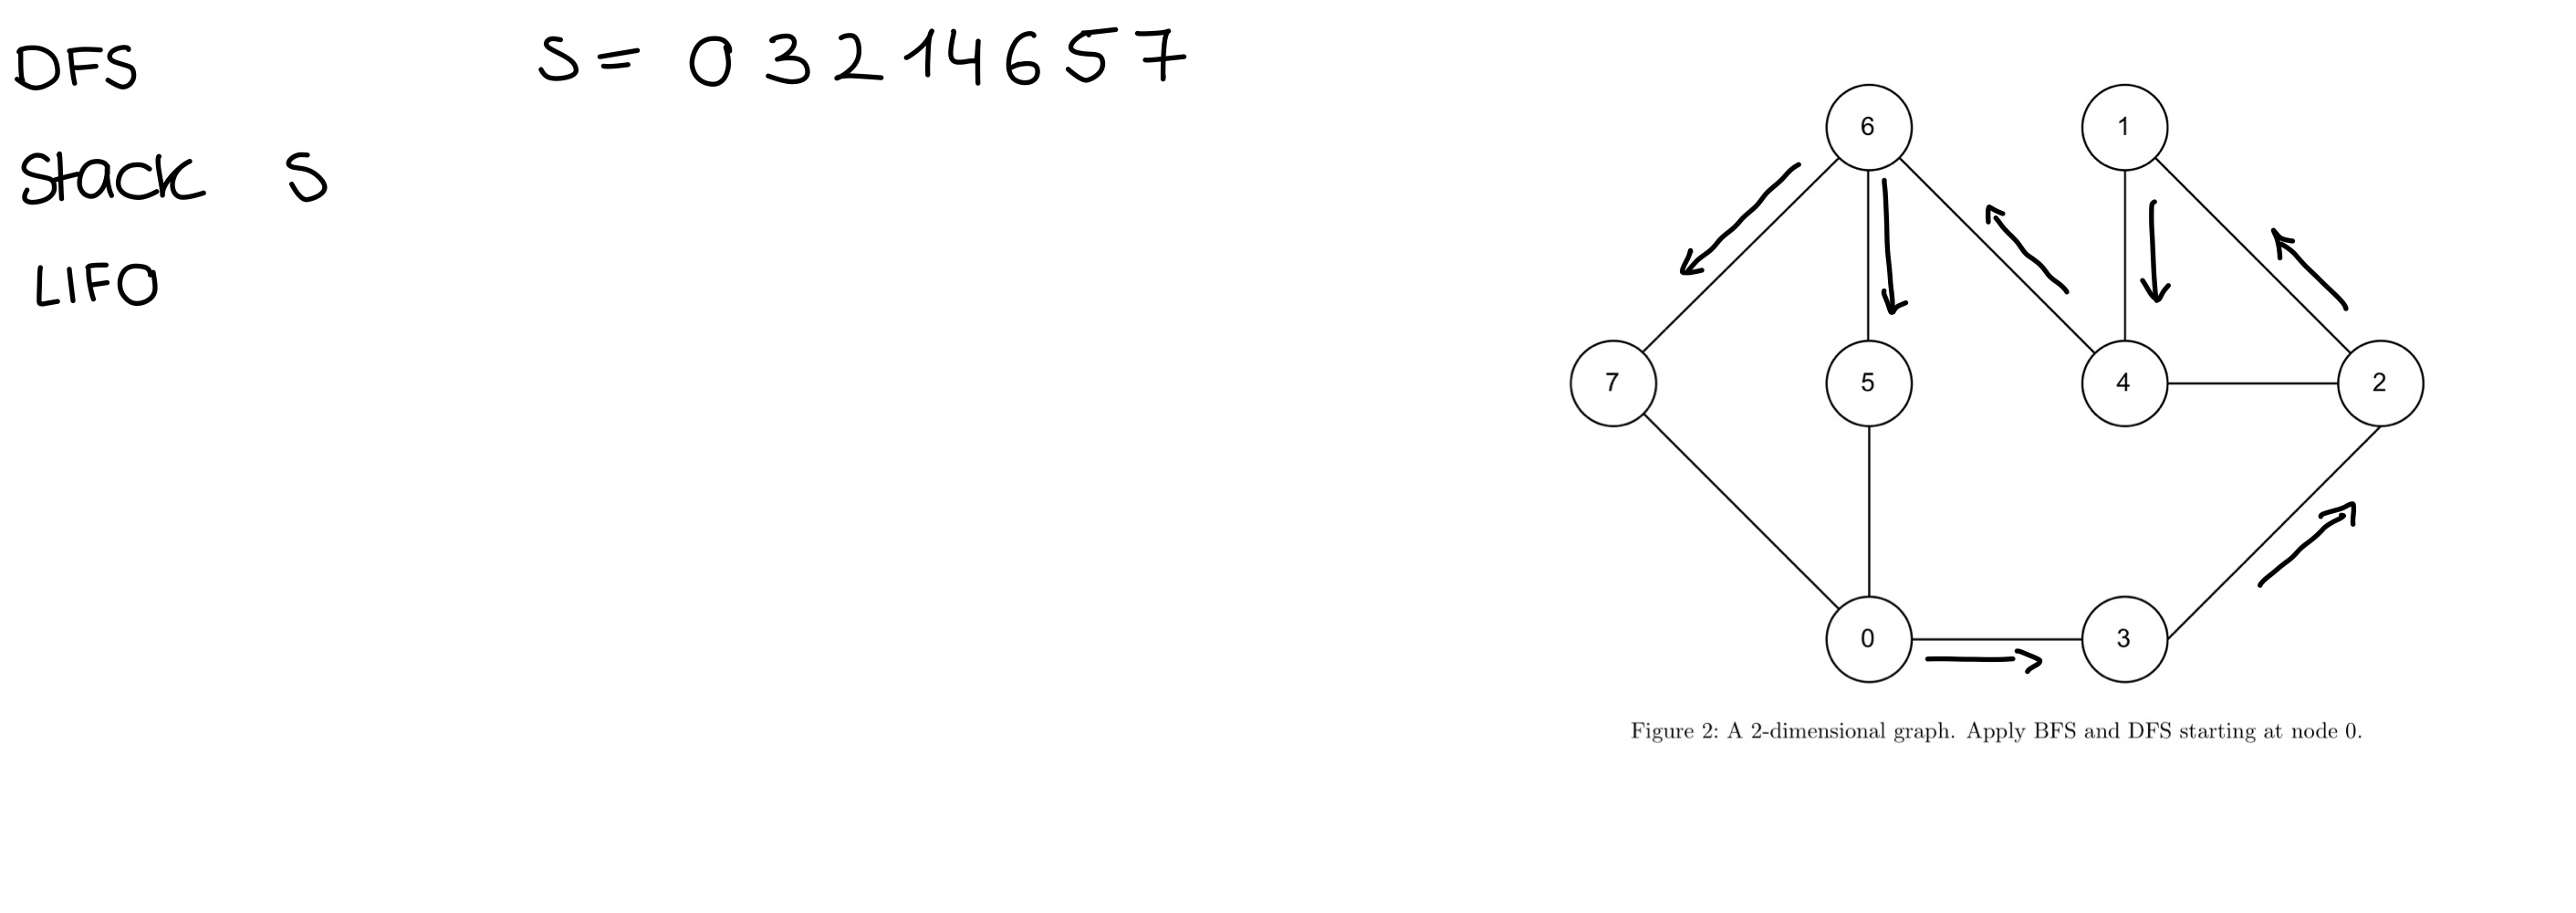
\includegraphics[width=\textwidth]{FAI6b.png}

    \subsection*{b) DFS - highest value first}
    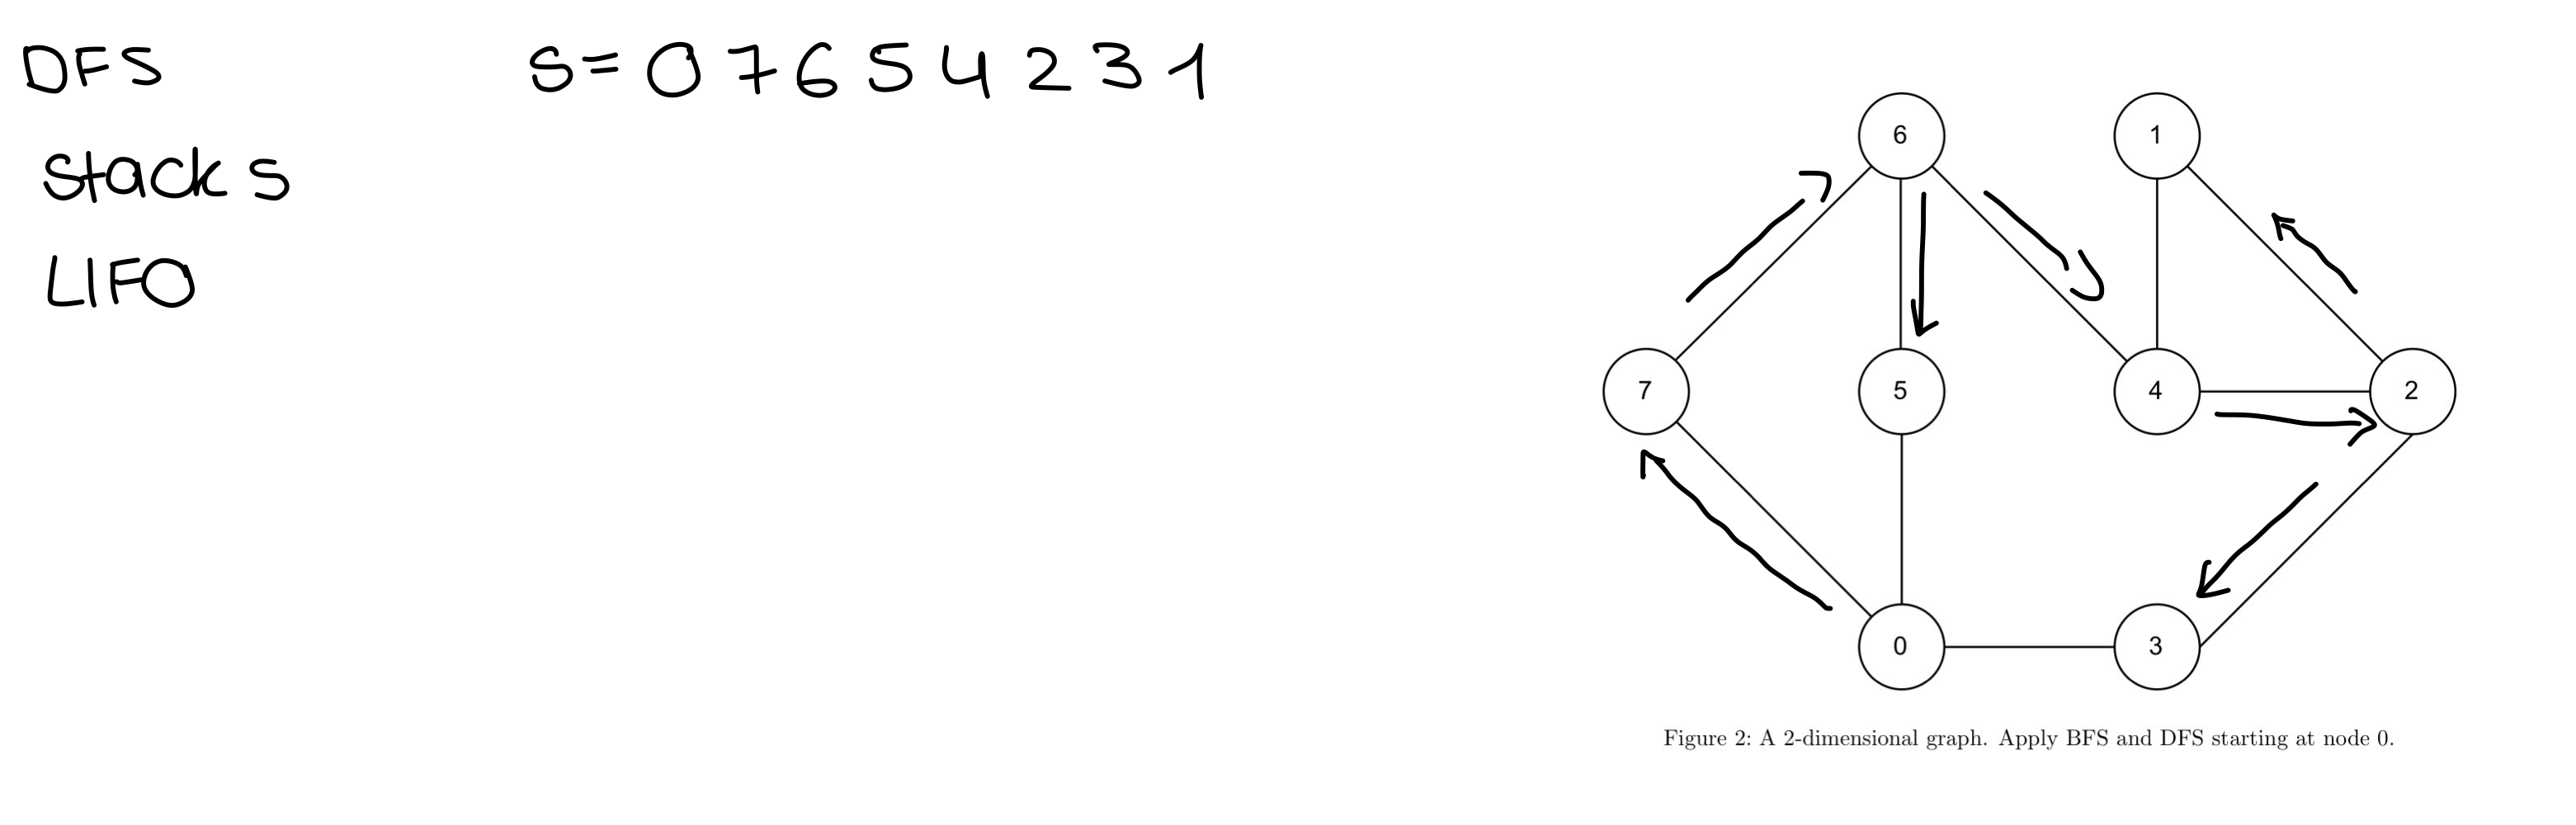
\includegraphics[width=\textwidth]{FAI6c.png}

\end{document}
